\documentclass[a4paper,12pt,italian]{article}
\usepackage{babel}
\usepackage[T1]{fontenc}
\usepackage[utf8]{inputenc}
\usepackage{amsmath}
\usepackage[margin=1.5cm]{geometry}
\usepackage{graphicx}

\title{
    Controlli Automatici T \\
    \large Progetto gruppo AO --- Traccia 3A\\
}
\author{
    Giacomo Romanini\\
    \and
    Guglielmo Palaferri\\
    \and
    Luca Tacinelli\\
    \and
    Pietro Girotti\\
}
\date{30 giugno 2021}

\begin{document}
\maketitle

\begin{figure}[h]
    \begin{center}
        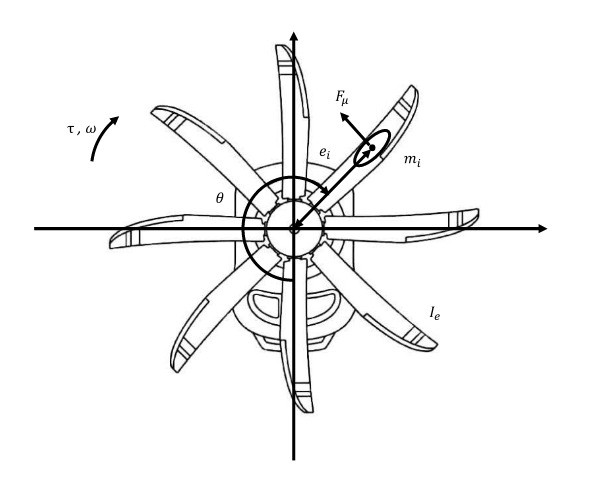
\includegraphics[scale=0.5]{img/elica.png}
        %\caption{Rappresentazione grafica del sistema (elica)}
    \end{center}    
\end{figure}

%\newpage

\section{Linearizzazione nell'intorno di $(x_e, u_e)$}
Il sistema del motore ad elica assegnato è descritto dalle seguenti equazioni: 

\begin{align*}
        \dot{\theta} &= \omega\\
        (m_i e_i^2 + I_e)\dot{\omega} &= -\beta \omega - \mu_d m_i \omega^2 e_i^2 + \tau
\end{align*}
Si considerano
\begin{align*}
    &x(t) =
    \begin{bmatrix}
        x_1(t)\\
        x_2(t)
    \end{bmatrix} =
    \begin{bmatrix}
        \theta(t)\\
        \omega(t)
    \end{bmatrix}\\
    &u(t) = \tau(t)\\
    &y(t) = \omega(t)
\end{align*}
Sostituendo i parametri è possibile ottenere le equazioni di stato:
\begin{equation*}
    \begin{aligned}
        \dot{x_1}(t) &= x_2(t)\\
        \dot{x_2}(t) &= -\frac{\beta}{(m_i e_i^2 + I_e)} x_2(t) - \frac{\mu_d m_i e_i^2}{(m_i e_i^2 + I_e)} x_2^2(t) + \frac{1}{(m_i e_i^2 + I_e)}u(t)
    \end{aligned}
\end{equation*} \\
Inoltre, poiché la dinamica di $\theta$ è ininfluente per l'evoluzione del sistema, si conosce $x_e = 
\begin{pmatrix}
    0\\
    10000/2\pi
\end{pmatrix}$
e $y_e = \omega_e = 10000/2\pi$.
$u_e$ può essere calcolato ponendo $f_2(x_e, u_e) = 0$:
\begin{equation*}
    -\beta x_{2e} - \mu_d m_i e_i^2 x_{2e}^2 + u_e = 0 \hspace{1em} \Longrightarrow \hspace{1em} u_e \approx 1110.7222
\end{equation*}
Si procede a questo punto calcolando le matrici del sistema linearizzato:
\begin{equation*}
    \delta \dot{x}(t) = A\delta x(t) + B\delta u(t)
\end{equation*}
\begin{equation*}
    \begin{array}{ll}
    A = \frac{\partial f(x,u)}{\partial x} \bigg|_{\substack{x=x_e\\u=u_e}} =
    \begin{bmatrix} 
        0 & 1 \\ 
        0 & - \frac{\beta}{m_ie_i^2 + I_e} - \frac{\mu_dm_ie_i^2}{m_ie_i^2 + I_e} 2\omega_e 
    \end{bmatrix}
    &B = \frac{\partial f(x,u)}{\partial u} \bigg|_{\substack{x=x_e\\u=u_e}} = 
    \begin{bmatrix} 
        0 \\ 
        \frac{1}{m_ie_i^2 + I_e}
    \end{bmatrix}\\ \\
    C = \frac{\partial h(x,u)}{\partial x} \bigg|_{\substack{x=x_e\\u=u_e}} =
    \begin{bmatrix} 
        0 & 1
    \end{bmatrix}
    &D = \frac{\partial h(x,u)}{\partial u} \bigg|_{\substack{x=x_e\\u=u_e}} =
    \begin{bmatrix} 
        0
    \end{bmatrix}
    \end{array}
\end{equation*}

%\newpage

\section{Funzione di trasferimento}

Per calcolare la funzione di trasferimento, si utilizza l'espressione
\begin{equation*}
    G(s) = C(sI + A)^{-1}B + D
\end{equation*}
dove
\begin{equation*}
    (sI - A)^{-1} = \frac{adj(sI - A)}{det(sI - A)} = 
    \begin{bmatrix}
        1/s & \frac{1}{s(s + 1.4139)} \\ 
        0   & \frac{1}{s + 1.4139}
    \end{bmatrix}
\end{equation*}
Ottenendo quindi la funzione di trasferimento:
\begin{equation*}
    G(s) =
    \begin{bmatrix}0 & 1 \end{bmatrix}
    \begin{bmatrix}
        1/s & \frac{1}{s(s+1.4139)} \\
        0 &\frac{1}{s+1.4139} \end{bmatrix}
    \begin{bmatrix}0 \\ 1.2903 \end{bmatrix}
    + 0 =
    \frac{1.2903}{s + 1.4139}
\end{equation*}
Avendo un polo in $s = -1.4139$, è possibile constatare con certezza che il sistema sia BIBO stabile.\\ \\
Di seguito il diagramma di Bode della funzione di trasferimento, ricavato tramite MATLAB.

\begin{figure}[h!]
    \begin{center}
        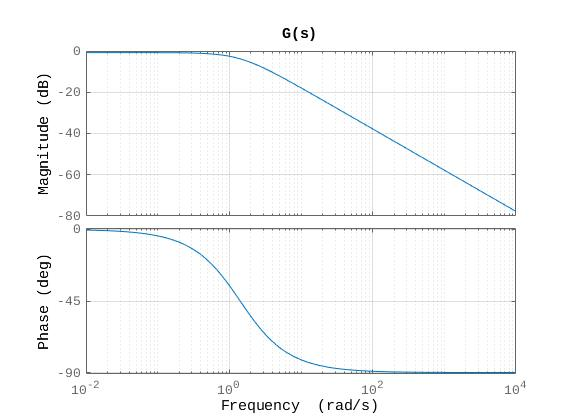
\includegraphics[scale=0.55]{img/bode_GG.jpg}
        %\caption{Rappresentazione grafica del sistema (elica)}
    \end{center}    
\end{figure}

\newpage

\section{Sintesi del regolatore}

\textbf{(3.1)} Per ottenere un errore a regime nullo con riferimento a gradino $w(t) = W1(t)$, $L(s)$ deve presentare un polo nell'origine.
Avendo un unico polo reale negativo, introduciamo un regolatore statico con un polo nell'origine: $ R_s(s) = \frac{1}{s} $ ricavandone quindi $ G_e(s) $:

\begin{equation*}
    G_e(s) = R_s(s)G(s) = \frac{1}{s}\Big(\frac{1.2903}{s + 1.4139}\Big)
\end{equation*}

\begin{figure}[h!]
    \begin{center}
        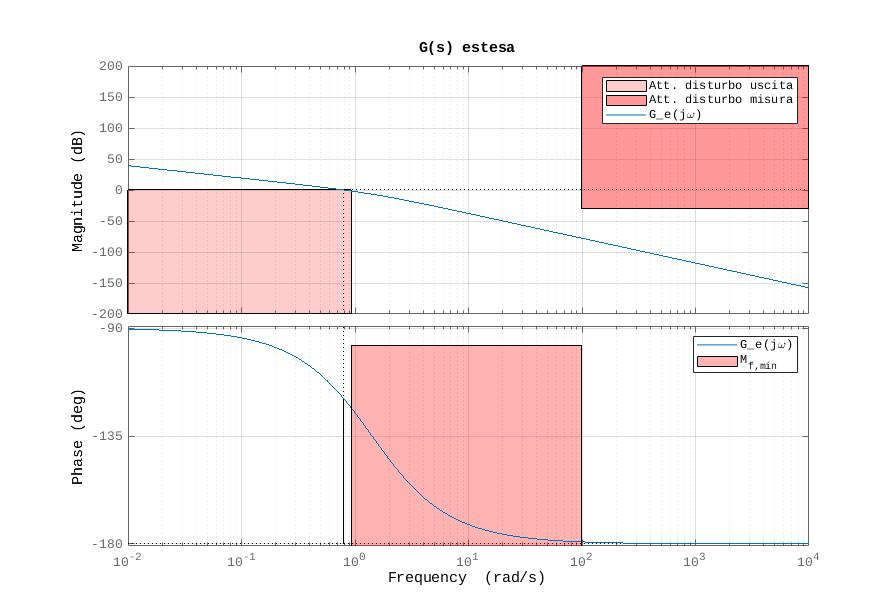
\includegraphics[scale=0.5]{img/bode_GG_estesa.jpg}
    \end{center}    
\end{figure}

\textbf{(3.2)} Come si può notare, il sistema esteso rispetta le specifiche iniziali sul margine di fase ($ M_f \geq 45^\circ$)\\

\textbf{(3.3)} La sovraelongazione percentuale massima accettabile è pari all'1\%. 
Da questo ricaviamo un nuovo vincolo sul margine di fase, sapendo che $M_f = \xi \cdot 100 $

\begin{equation*}
    \begin{array}{c}
        \xi^* = \sqrt{\frac{(ln(0.01))^2}{\pi^2+(ln(0.01))^2}} = 0.8261\\ \\
        M_f=\xi * 100 \Longrightarrow M^*_{f,min}=0.8261 \cdot 100 = 82.61
        \Longrightarrow arg(L(j\omega_c)) \geq -97.39^\circ
    \end{array}
\end{equation*}\\
Il nuovo vincolo sul margine di fase introduce quindi un minimo non rispettato dal sistema esteso.\\

\textbf{(3.4)} Il tempo di assestamento all'1\% deve essere mantenuto al di sotto dei 6 secondi.
Posso quindi ottenere $ \omega_{c,min} $

\begin{equation*}
    T_{a,1} = 6 
    \Longrightarrow 
    \omega_c \ge \frac{460}{6 \cdot 82.61}
    \Longrightarrow
    \omega_c \ge 0.9281
\end{equation*}

\newpage

\textbf{(3.5)} Considerando variazioni del parametro $e_i$ di $\pm 0.1$, si ottiene il seguente grafico:

\begin{figure}[h!]
    \begin{center}
        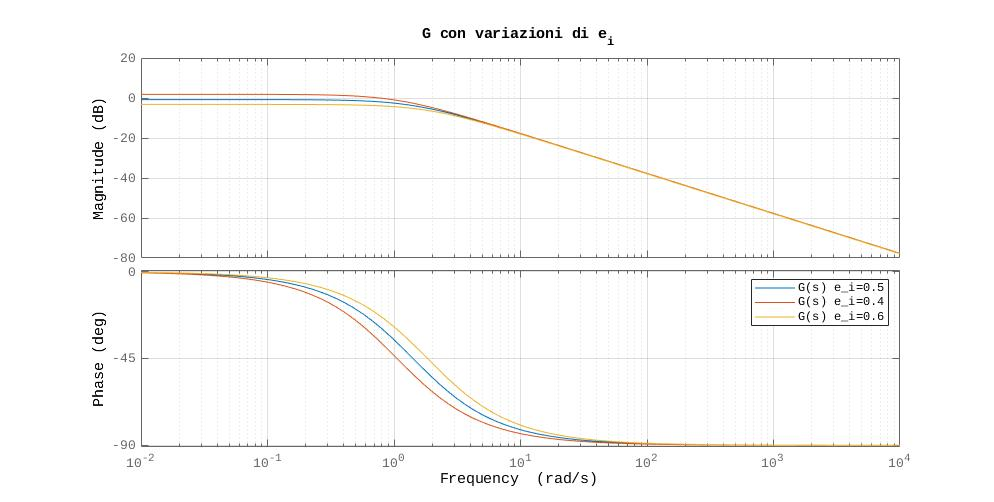
\includegraphics[scale=0.5]{img/bode_GG_ei.jpg}
    \end{center}    
\end{figure}

\section{Disturbo di misura}

Il disturbo di misura presenta componenti frequenziali $\geq 100 rad/s$ e deve essere abbattuto di almeno 30 volte.
Di conseguenza a frequenze $\omega \geq 100 rad/s$, il grafico di $L(j\omega)$ non potrà avere ampiezze maggiori di $-30dB$



\end{document}